\documentclass{beamer}

\mode<presentation> {




%\usetheme{Antibes} %ok
%\usetheme{Berlin} %ok
%\usetheme{Boadilla} %ok
\usetheme{Darmstadt} %ok
%\usetheme{Dresden} %ok
%\usetheme{Frankfurt} %ok
%\usetheme{Ilmenau} %ok
%\usetheme{Pittsburgh} %ok
%\usetheme{Rochester} %ok


%\usecolortheme{dolphin}
%\usecolortheme{orchid}
%\usecolortheme{whale}



}


\usepackage[utf8]{inputenc}
\usepackage[OT4]{polski}
\usepackage{tabularx}

\usepackage{graphicx} % Allows including images
\usepackage{booktabs} % Allows the use of \toprule, \midrule and \bottomrule in tables



\title[Modelowanie klimatu]{Modelowanie klimatu} % The short title appears at the bottom of every slide, the full title is only on the title page

\author{Axel Zuziak, Marcin Węglarz} % Your name
\institute[AGH WFiIS]
{
AGH WFiIS \\
Fizyka Techniczna\\ % Your institution for the title page
\medskip
}
\date{\today} % Date, can be changed to a custom date

\begin{document}
%progress bar in footline *************************************************************************

\definecolor{lightgr}{rgb}{0 0.4 0.9}
\makeatletter
\addtobeamertemplate{footline}{%
	\color{lightgr}% to color the progressbar
	\hspace*{-\beamer@leftmargin}%
	%\rule{\beamer@leftmargin}{0pt}%
	\rlap{\rule{\dimexpr
			\beamer@startpageofframe\dimexpr
			\beamer@rightmargin+\textwidth\relax/\beamer@endpageofdocument}{3pt}} %grubosc paska
	% next 'empty' line is mandatory!
	
	\vspace{0\baselineskip}
	{}
} %koniec progress bara **************************************************************************************



%++++++++++++++++++++++++++++++++++++++++++++++++++++++++++++++++++++++++
%notatki
%str 47-63
%str 117-150
%str 165-200
%str 244-246

%++++++++++++++++++++
%s.176
%TODO
%Fizyka + równania
%Implementacja tych równań 
%Typy modeli (0,1,2,3 wymiarowe + kompletne)
%s.60








\begin{frame}
\titlepage % Print the title page as the first slide
\end{frame}

%\begin{columns}[c]
%\column do  robienia kolumn
%\end{columns}

%\begin{frame}
%\frametitle{Overview} % Table of contents slide, comment this block out to remove it
%\tableofcontents % Throughout your presentation, if you choose to use \section{} and \subsection{} commands, these will automatically be printed on this slide as an overview of your presentation
%\end{frame}

%----------------------------------------------------------------------------------------
%	PRESENTATION SLIDES
%----------------------------------------------------------------------------------------

%------------------------------------------------
%\section{First Section} % Sections can be created in order to organize your presentation into discrete blocks, all sections and subsections are automatically printed in the table of contents as an overview of the talk
%------------------------------------------------

%\subsection{Subsection Example} % A subsection can be created just before a set of slides with a common theme to further break down your presentation into chunks

\begin{frame}
\frametitle{Co to jest klimat?}
Klimatem nazywamy średnie warunki pogodowe obserwowane w danym miejscu na przestrzeni lat. Przykładowe czynniki: temperatura, opady, zachmurzenie, wilgotność.
Modele klimatu są uproszonym opisem skomplikowanych procesów.
Klimat dzielimy na pięć części:
\begin{itemize}
	\item \textbf{Atmosfera} Gazowa część ponad powierzchnią ziemi.
	\item \textbf{Hydrosfera} Wszystkie formy wody nad i pod powierzchnią ziemi.
	\item \textbf{Kriosfera} Wszystkie formy wody w postaci lodu.
	\item \textbf{Powierzchnia lądowa}
	\item \textbf{Biosfera} Organizmy żyjące w hydrosferze oraz na powierzchni lądowej.
\end{itemize}
\end{frame}


\begin{frame}
	\frametitle{}
	\begin{figure}[h]
		\begin{center}
			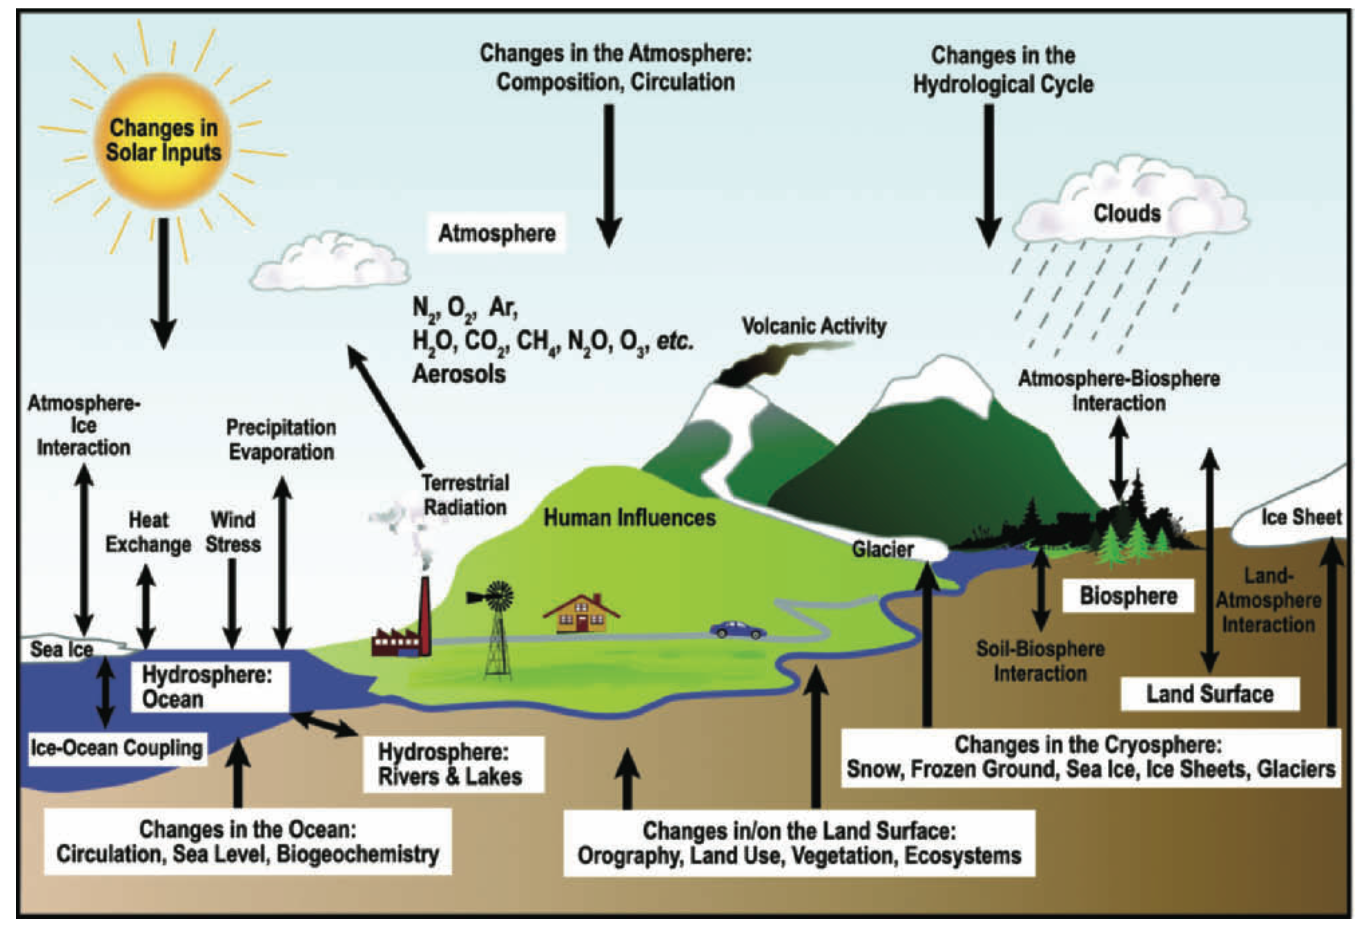
\includegraphics[width=0.7\linewidth]{images/Figure1}
			\caption{Czynniki definiujące i wpływające na klimat}
		\end{center}
	\end{figure}
\end{frame}

\begin{frame}
	\frametitle{Zerowymiarowy model cieplarniany}
	\begin{figure}[h]
		\begin{center}
			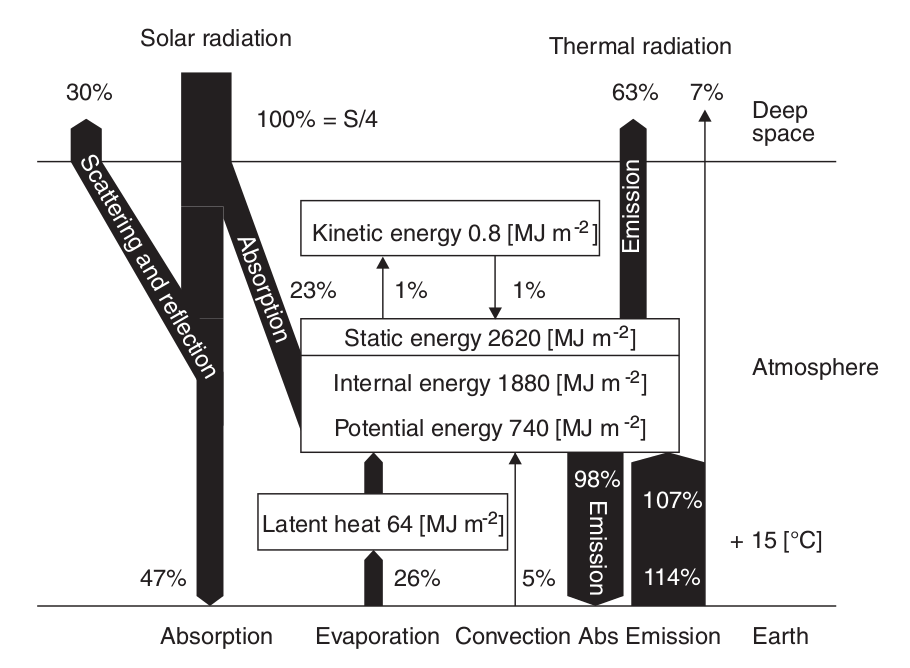
\includegraphics[width=0.7\linewidth]{images/0D_Model.png}
			\caption{Zerowymiarowy model bilansu promieniowania}
		\end{center}
	\end{figure}

\end{frame}



\begin{frame}
	\frametitle{Matematyczne spojrzenie na bilans energetyczny}
	\begin{block}{Bardzo prosty model bilansu radiacyjnego}
		\[(1-a)\frac{S}{4} = \sigma T_a^4 + t\sigma T_s^4
		\]
	\end{block}
	\begin{block}{Bilans dla powierzchni Ziemi}
		\[(-t_a)(1-a_s)\frac{S}{4}+c(T_s - T_a)+\sigma T_a^4 =0
		\]
	\end{block}
	\begin{block}{Bilans dla atmosfery}
		\[-(1- a_a-t_a+a_st_a)\frac{S}{4} - c(T_s - T_a) - \sigma T_s^4
		(1-t_a^{'}-a_a^{'}) + 2\sigma T_a^4=0
		\]
	\end{block}
	%Literką \it{a} oznaczamy albedo, natomiast \it{t} oznacza przepuszczalność. 
	%odpowiednie indeksy oznaczają wartość dla atmosfery(a) lub powierzchni Ziemi(s).
	\scriptsize{(Wartości z primem to wartości dla fal długich.)}
	
\end{frame}

\begin{frame}
	\frametitle{Hipotetyczne przykłady}
	\begin{itemize}
		\item \textit{Współczesna Ziemia.} ($a=0,30, T_s=288K$)
		\item \textit{Biała Ziemia.} ($a = 0,50;T_s=268K$)
		\item \textit{Zima nuklearna.} ($a=0,35; T_s=284K$)
	\end{itemize}
	
\end{frame}

\begin{frame}
	\frametitle{Wymuszenie radiacyjne i sprzężenie zwrotne.}
	\textbf{Wymuszeniem radiacyjnym} nazywamy zjawisko zmiany temperatury na powierzchni Ziemi celem wyrównania bilansu radiacyjnego. 
	\begin{block}{Wzory do ilościowego opisu zmian temperatury}
		\[\Delta I = \frac{\partial I}{\partial T_s}\Delta T_s
		\]
		\[\frac{\partial I}{\partial T_s} = \frac{4}{T_s}(1-a)\frac{S}{4}
		\]
		
		%z tego modelu dI 3,1 W/m(-2)K(-1)
		%z dokladniejszych 4,6 - efekt uwzglednienia sprzezenia zwrotnego
	\end{block}
\end{frame}


\begin{frame}
	\frametitle{Przykłady zjawisk wpływających na globalne ocieplenie}

	\textbf{Zjawiska mogące wzmagać globalne ocieplenie:}
	\begin{enumerate}
		\item Topienie się lodów i śniegów.
		
		\item Zwiększenie ilości pary wodnej w powietrzu. 
		($t_a^{'}\nearrow; a_a^{'}\searrow$).
		
		\item Wzrost zachmurzenia.
		
		\item Wzrost $CO^2$ (mniejsza absorpcja przez oceany,
		szybszy rozkład materii).
		
		\item Szybszy wzrost roślin i zmiana albedo.

	\end{enumerate}

\end{frame}


\begin{frame}
	\frametitle{Przykłady zjawisk wpływających na globalne ocieplenie}
	
	\textbf{Zjawiska mogące osłabiać globalne ocieplenie:}
	
	\begin{enumerate}
		
		\item Wzrost zawartości pary wodnej (średni spadek temperatury
		z wysokością maleje).
		
		\item Wzmożony rozwój alg we wszystkich wodach (użycie $CO^2$ 
		do fotosyntezy).
		
	\end{enumerate}
	
\end{frame}



\begin{frame}
	\frametitle{Opóźnienie czasowe ze względu na obecność oceanów}
	
	\begin{itemize}
		\item Wysoka pojemność cieplna wody.
		
		\item Duża powierzchnia wód na Ziemi.
		
		\item Powolne zmiany temperatury.
	
	\end{itemize}
	
	\begin{block}{Zmiana temperatury w wyniku wymuszenia radiacyjnego}
		\[\Delta T_s(t) = G_f\Delta I
		\]
	\end{block}
	
	\begin{block}{Ta sama zmiana po uwzględnieniu opóźnienia czasowego}
		\[\Delta T_s(t) = G_f\Delta I(1-\exp^{-t/\tau _e})
		\]
	\end{block}
	
	$\tau _e \approx 50-100$ lat
	
\end{frame}






\begin{frame}
	\frametitle{Implementacja}
	W celu implementacji naszych równań musimy im nadać wartości dyskretne.
	Modelujemy atmosferę, dzieląc ją na pudła.
	
	\begin{figure}[h]
		\begin{center}
			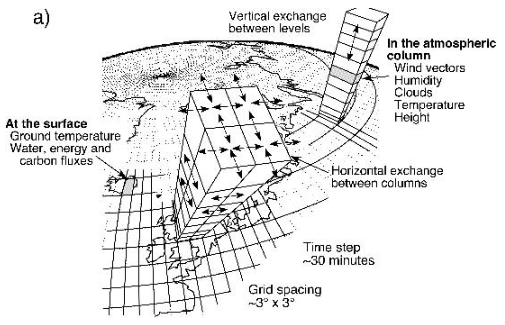
\includegraphics[width=0.7\linewidth]{images/box.png}
			\caption{Model podziału atmosfery na pudła.}
		\end{center}
	\end{figure}
	
	%zajrzec na strone 170 \cite{b1} spectral model - nie wiem czy mowic o tym
	%strona 187 opis 6 zmiennych i 6 rownan je opisujacych
\end{frame}



\begin{frame}
	\frametitle{Modele klimatu}
	Ogólnie możemy podzielić na modele:
	\begin{itemize}
		\item zerowymiarowe
		\item 1-wymiarowe
		\item 2-wymiarowe
		\item 3-wymiarowe
	\end{itemize}
	\vspace{0.5cm}
	Spośród powyższych najdokładniejsze są modele 3-wymiarowe, z których należy wyróżnić
	\begin{itemize}
		\item GCM (general circulation model), AGCM,OGCM,CGCM lub AOGCM
		\item RCM (regional climate model)
	\end{itemize}

		

\end{frame}


\begin{frame}
	\frametitle{TODO}
	\begin{itemize}
		\item Zmienne w modelach
		\item Opisać modele 0/1/2/3 wymiarowe
		\item Problemy i sprzężenia zwrotne
		\item Modelowanie atmosfery, oceanu, lądu, innych
	\end{itemize}
\end{frame}


\begin{frame}
	\frametitle{Plan prezentacji}
	\begin{enumerate}
		\item Co to jest klimat.
		\item Ważne pojęcia.
		\item Model zerowymiarowy - rozgrzewka (???).
		\item Modelowane zjawiska fizyczne (atmosfera, ocean ...).
		\item Sprzężenia zwrotne i parametryzacja.
		\item Rodzaje modeli + streszczenie.
		\item Implementacja GCM.
	\end{enumerate}
\end{frame}




\begin{frame}
	\frametitle{Modelowanie oceanu}
	TODO
	
\end{frame}


\begin{frame}
	\frametitle{Modelowanie kriosfery}
	TODO
	
\end{frame}


\begin{frame}
	\frametitle{Modelowanie powierzchni ziemi}
	TODO
	
\end{frame}


\begin{frame}
	\frametitle{Modelowanie zjawisk chemicznych w atmosferze}
	TODO
	
\end{frame}



\begin{frame}
	\frametitle{Modelowanie atmosfery}
	\begin{block}{Prawo zachowania pędu}
		
		\[\frac{D\mathbf{v}}{Dt} = -2 \mathbf{\Omega} \times \mathbf{v} - \rho^{-1}
		\nabla p + \mathbf{g} + \mathbf{F}
		\]
		
	\end{block}
	
	\begin{block}{Prawo zachowania masy}
		\[\frac{D\rho}{Dt} = -\rho\nabla \cdot \mathbf{v} + C - E
		\]
	\end{block}
	
	\begin{block}{Prawo zachowania energii}
		\[\frac{DI}{Dt} = -p\frac{D\rho^{-1}}{Dt} + Q
		\]
	\end{block}
	
	\begin{block}{Równanie stanu gazu doskonałego}		
		\[p=\rho RT
		\]
	\end{block}
	
	
\end{frame}



\begin{frame}
	\frametitle{Modele 1D/2D/3D}
	\begin{enumerate}
		\item Model 1D:
		\begin{itemize}
			\item Model RC (radiative-convectiv model). %s.131
			\item One-dimensional EBM (energy balance model). %s.95
		\end{itemize}
		
		\item Model 2D:
		\begin{itemize}
			\item Two-dimensional SD (statistical dynamical) climate model.
			%height in the atmosphere and latitude
			%zonally averaged values
		\end{itemize}
		
		\item Model 3D:
		\begin{itemize}
			\item GCM (general circulation model)
		\end{itemize}
	\end{enumerate}
	
	
	
	
\end{frame}


\begin{frame}
	\frametitle{Przykład modelowania 2D}
	
	\begin{figure}[h]
		\begin{center}
			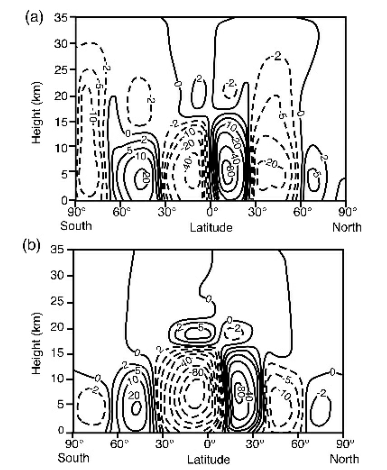
\includegraphics[width=0.4\linewidth]{images/2D_model.png}
			\caption{Rysunek przedstawia średni roczny przepływ masy. a) obserwowany, b) przewidziany modelem}
		\end{center}
	\end{figure}
	
	
\end{frame}








\begin{frame}
\frametitle{References}
\footnotesize{
\begin{thebibliography}{99} % Beamer does not support BibTeX so references must be inserted manually as below
\bibitem[McGuffie]{b1} K.McGuffie, A. Henderson-Sellers
\newblock A Climate Modelling Primer

\end{thebibliography}
}
\end{frame}


\begin{frame}
\Huge{\centerline{The End}}
\end{frame}


\end{document} 